\subsection{Der spezifische Workflow}\label{l:workflow}

\begin{figure}[htb]
\begin{center}
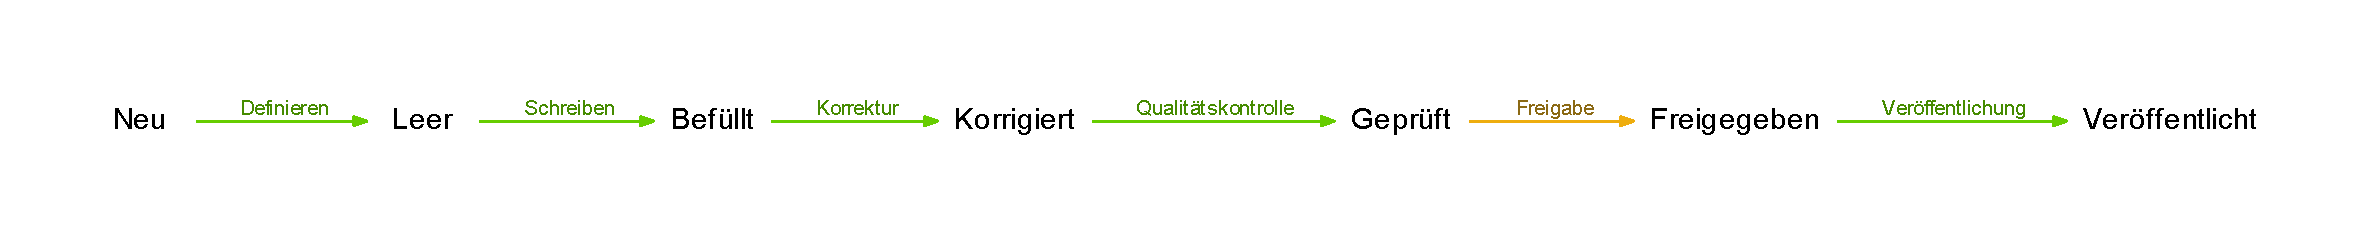
\includegraphics[width=\textwidth]{media/chart-3.pdf}
\end{center}
\caption{Operationen bei der Erstellung von Texten}
\label{chart:3}
\end{figure}

\paragraph{\emph{Wie} wird Einfluss auf den Workflow genommen} Beobachtet man verschiedene Projekte, in denen Informations- und Kommunikationsmedien erstellt werden, lässt sich feststellen, dass Texte immer wieder auf die gleiche Art beeinflusst werden. Für eine vollständige Beschreibung des Workflows ist es zunächst sinnvoll, zu ermitteln, \emph{wie} Texte beeinflusst werden. 

Betrachtet man die Arbeiten in Zusammenhang mit Text lassen sich diese in sechs eigenständige Operationen unterteilen, die in Abbildung~\ref{chart:3} in Zusammenhang dargestellt sind:

\begin{enumerate}
\item{Durch \textbf{Definieren eines Textbausteines} werden dessen Attribute bestimmt. Dadurch wird festgelegt, wie der benötigte Text beschaffen sein muss. Die Aussage \citequotes{Wir brauchen an dieser Stelle eine Überschrift} ist ein Beispiel für diese Operation. Sie legt fest, wie der Textbausteine gestaltet werden muss, um die ihm zugedachte Aufgabe zu erfüllen. Neben der Angabe zur Platzierung auf dem Medium durch \typoquotes{an dieser Stelle} wird implizit durch \typoquotes{eine Überschrift} eine Angabe zur inhaltlichen und visuellen Gestaltung getroffen; Überschriften sollen kurz und knapp sein und ihre visuelle Gestaltung wird durch den Styleguide des Projektes festgelegt.}
\item{Das \textbf{Schreiben eines Textes} erzeugt den Inhalt eines Textbausteins in einer Sprache. Bei diesem Vorgang wird der Text entsprechend der Vorgabe aus der Beschreibung als Original erstellt oder aus Quellen außerhalb des Projektes kopiert und eingefügt. }
\item{In der \textbf{Korrektur} wird der Text inhaltlich und grammatikalisch überprüft und entsprechend angepasst. Der Korrektor muss dabei für eine grammatikalische Überprüfung des Textes kein Fachwissen bezogen auf das Projekt haben. Ist diese Fachwissen vorhanden, kann eine inhaltliche Korrektur vorgenommen werden.}
\item{In der \textbf{Qualitätskontrolle} wird der Text dahingehend überprüft, ob er den Anforderungen gemäß der Beschreibung und inhaltlichen Vorgaben, auch hinsichtlich des gesamten Projektes entspricht. Abbildung~\ref{chart:4} verdeutlicht den Einfluss der Qualitätskontrolle auf den Verlauf eines Projektes.}
\item{Durch die \textbf{Freigabe} wird der Text abgenommen und kann nun in das Endprodukt übernommen werden. Die Freigabe unterscheidet sich von der Qualitätskontrolle durch ihren authorativen Charakter. Qualitätskontrolle können prinzipiell von allen Mitarbeitern durchgeführt werden. Freigaben werden nur von Mitarbeitern mit Management-Berechtigungen erteilt.}
\item{Durch die \textbf{Veröffentlichung} wird der Text in das Endprodukt eingebracht.}
\end{enumerate}

\begin{figure}[htb]
\begin{center}
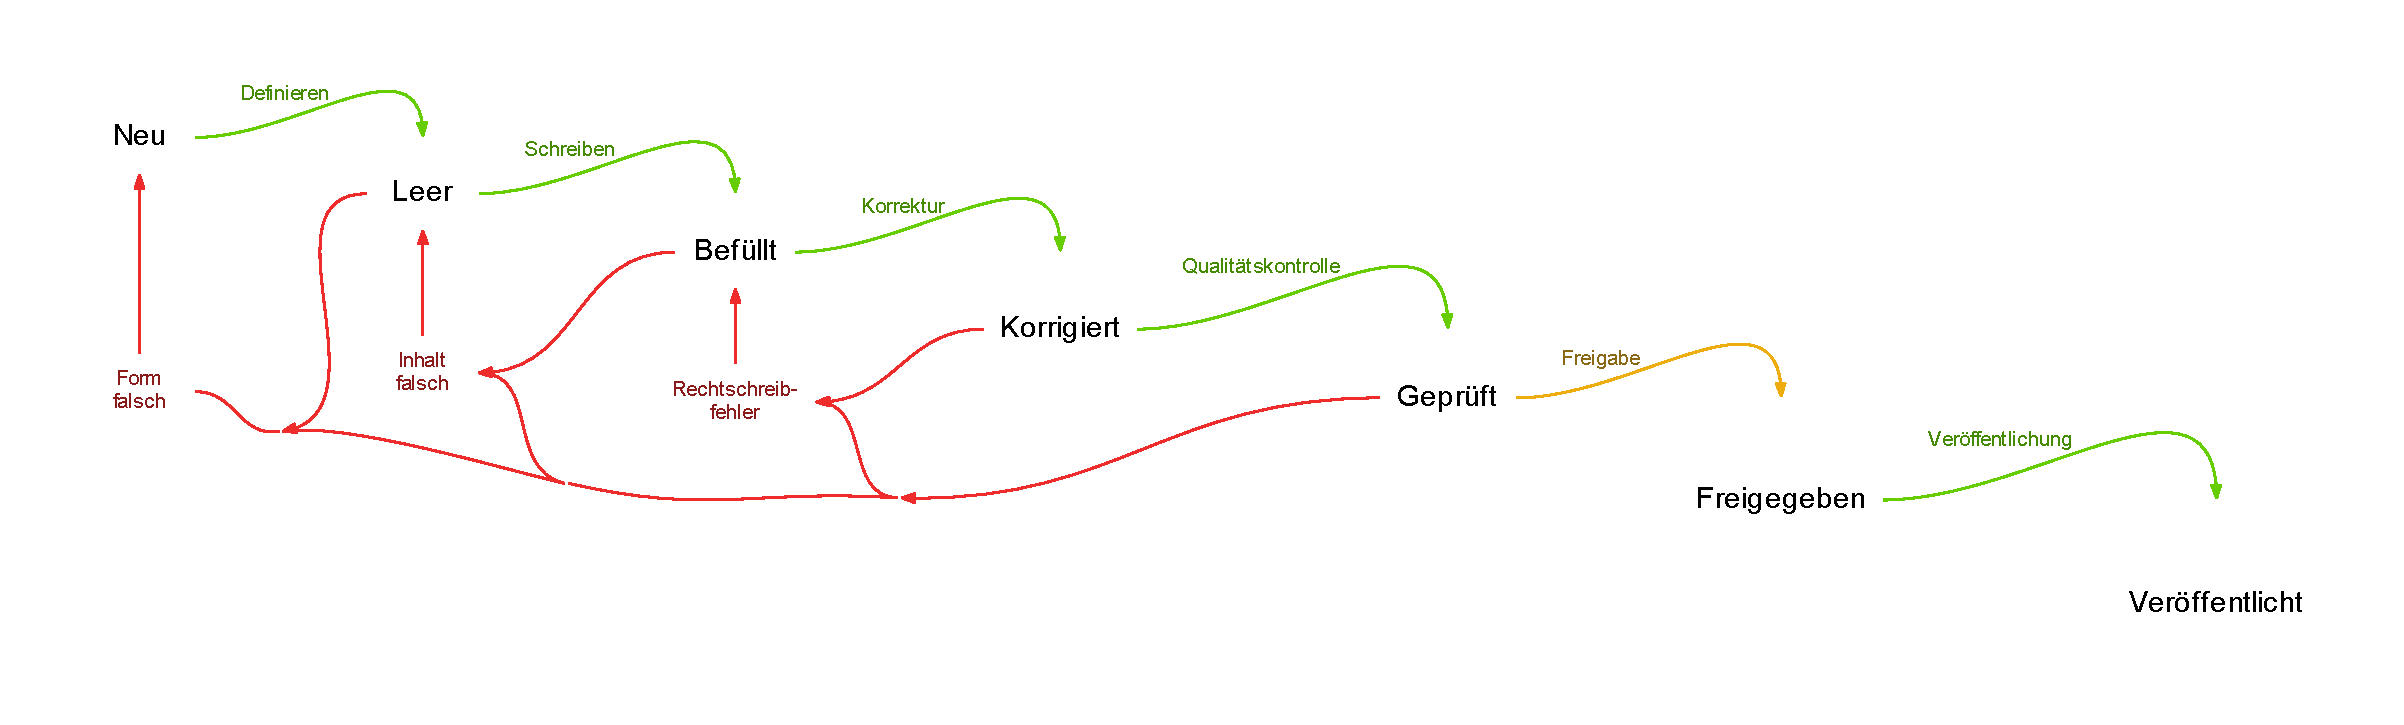
\includegraphics[width=\textwidth]{media/chart-4.pdf}
\end{center}
\caption{Operationen bei der Erstellung von Texten mit Qualitätskontrolle}
\label{chart:4}
\end{figure}

\paragraph{\emph{Wer} hat Einfluss auf den Workflow} In Abschnitt~\ref{l:besondererolle} ab Seite~\pageref{l:besondererolle} wurde bereits beschrieben, wie umfangreich die Anzahl der Personen ist, die Einfluss auf die Texte eines Produktes haben. Die Rollenverteilung ist dabei von Projekt zu Projekt unterschiedlich. Allen gemeinsam ist aber, dass die beteiligten Personen  Einfluss auf drei grundlegenden Eigenschaften von Text haben: den Inhalt des Textes, die Attribute wie z.B. \typoquotes{maximale Textlänge} oder \typoquotes{Position im Medium} und den Status wie z.B. \typoquotes{neu} und \typoquotes{freigegeben}. Anhand dieses Kriteriums lassen sich Mitarbeiter in drei Gruppen unterteilen. Tabelle~\ref{table:texteinfluss} zeigt dies in einer Übersicht. Personen die Einfluss auf den \emph{Inhalt} haben, sind vor allem diejenigen die die Texte für das Produkt liefern. Neben den Mitarbeitern auf Kundenseite, Ausgangsmaterialien und Fachinformationen zur Verfügung stellen sind die Texter und Übersetzer, die diese Informationen aufbereitet. Texte müssen aber auch die die spezifischen Gegebenheiten des Mediums angepasst werden , hierzu liefern Experten Rahmenbedingungen aber auch inhaltliche Anpassungen. Ein Beispiel hierfür ist die suchmaschinenoptimierung (SEO) von Texten. Hierbei werden Texte auf das vorhandensein von bestimmte Formulierungen und Stichwörter optimiert aber auch Vorgaben über die Länge und Aufbau von Texten gemacht. Attribute legen die Rahmenbedingungen von Text fest, diese werden vor allem in der Gestaltung des Produktes durch Designer, als auch in der Umsetzung durch produktbedingte Einschränkungen, z.B. Platzverhältnisse oder systembedingte Beschränkungen, bestimmt. Den Status von Texten, also ob ein Text dem nächsten Mitarbeiter im Workflow zugewiesen werden soll kann von bestimmten Mitarbeitern abhängen. Es ist üblich, dass Texte erst dann dem Kunden zur Abnahme vorgelegt werden, wenn sie als Gesamtes vorliegen. Auch externe Dienstleister bekommen aus Kostengründen meisten alle Text im Paket, damit eine zügige Abarbeitung des Auftrages gewährleistet wird.

\begin{table}
\begin{center}
\begin{tabular}{@{}r c c c}
\textbf{Person} & \textbf{Inhalt} & \textbf{Attribute} & \textbf{Status}\\
\hline
\textbf{Agentur} & & & \\
\hline
Projektleiter & --- & --- & \checkmark \\
Informationsarchitektur & --- & \checkmark & --- \\
Art-Direktion & --- & \checkmark & --- \\
Programmierer & --- & \checkmark & --- \\
\textbf{Extern} & & & \\
\hline
Texter & \checkmark & --- & --- \\
Lektorat & \checkmark & --- & --- \\
Übersetzungsbüro & \checkmark & --- & --- \\
SEO-Experte  & \checkmark & \checkmark & --- \\
\textbf{Kunde} & & & \\
\hline
Projektleiter & --- & --- & \checkmark \\
Fachabteilung & \checkmark & --- & --- \\
Rechtsanwalt  & \checkmark & --- & \checkmark \\
Marketingabteilung & \checkmark & --- & --- \\
\end{tabular}
\caption{Arten von Einfluss, die Mitarbeiter in einem Projekt haben}
\label{table:texteinfluss}
\end{center}
\end{table}

\begin{figure}[htb]
\begin{center}
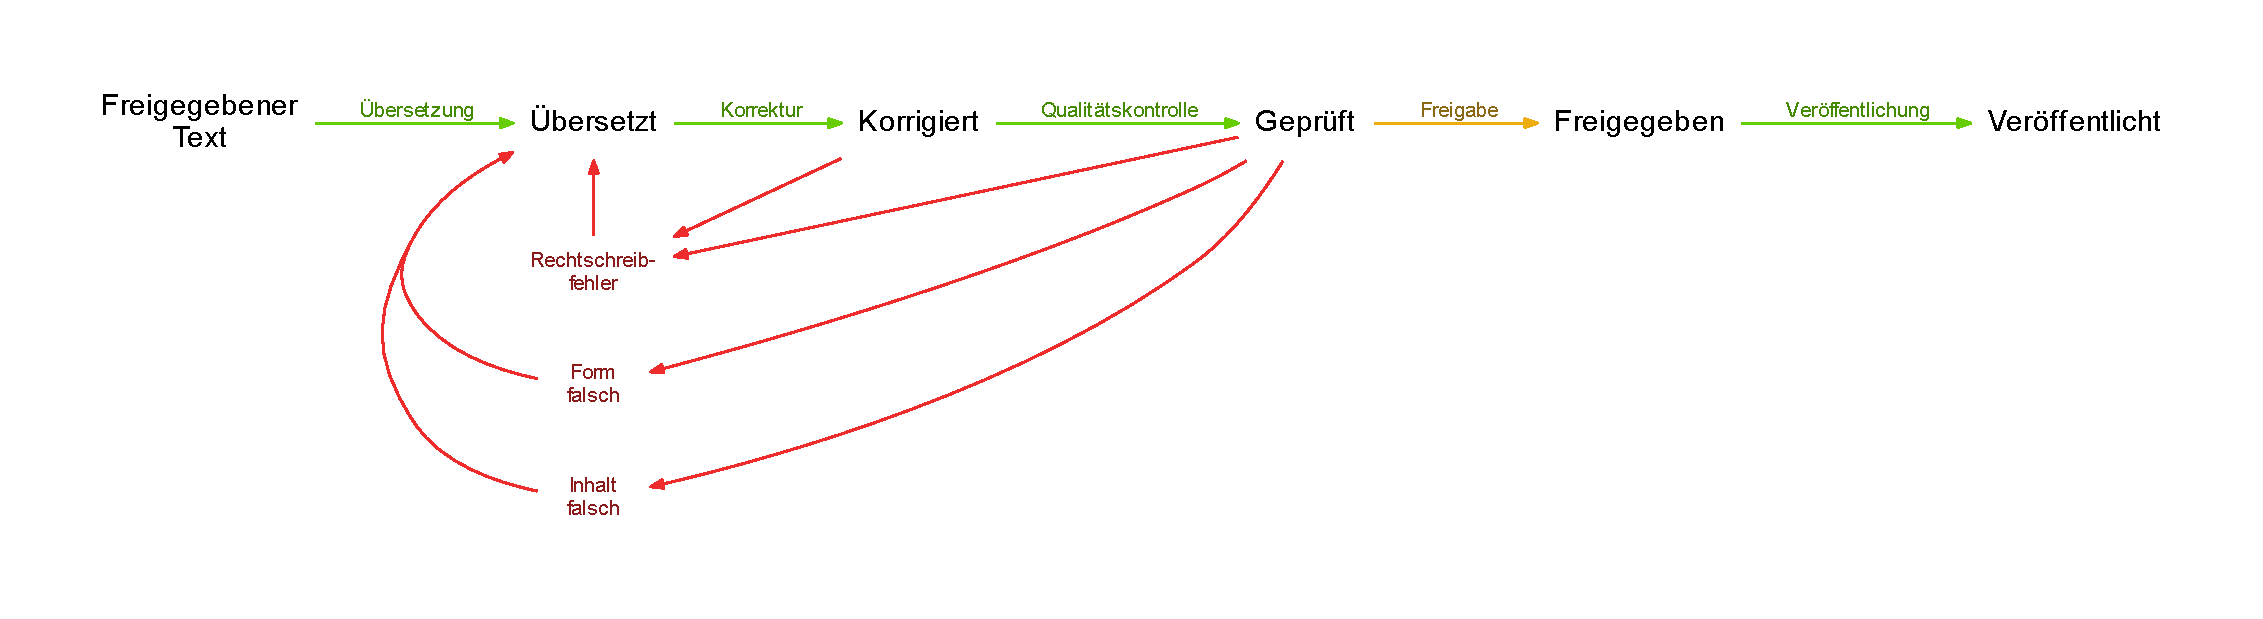
\includegraphics[width=\textwidth]{media/chart-5.pdf}
\end{center}
\caption{Operationen bei der Übersetzung von Texten mit Qualitätskontrolle}
\label{chart:5}
\end{figure}

Die bisher genannten Abläufe lassen sich auch 1:1 auf die Übersetzung von Texten anwenden. Abbildung~\ref{chart:5} zeigt den Workflow schematisch.

Abbildung~\ref{chart:personas-gewichtet}~(S.\pageref{chart:personas-gewichtet}) zeigt diese Beziehungen in einem, nach Anzahl der Kommunikationspartner gewichteten Graphen

\begin{figure}[htb]
\begin{center}
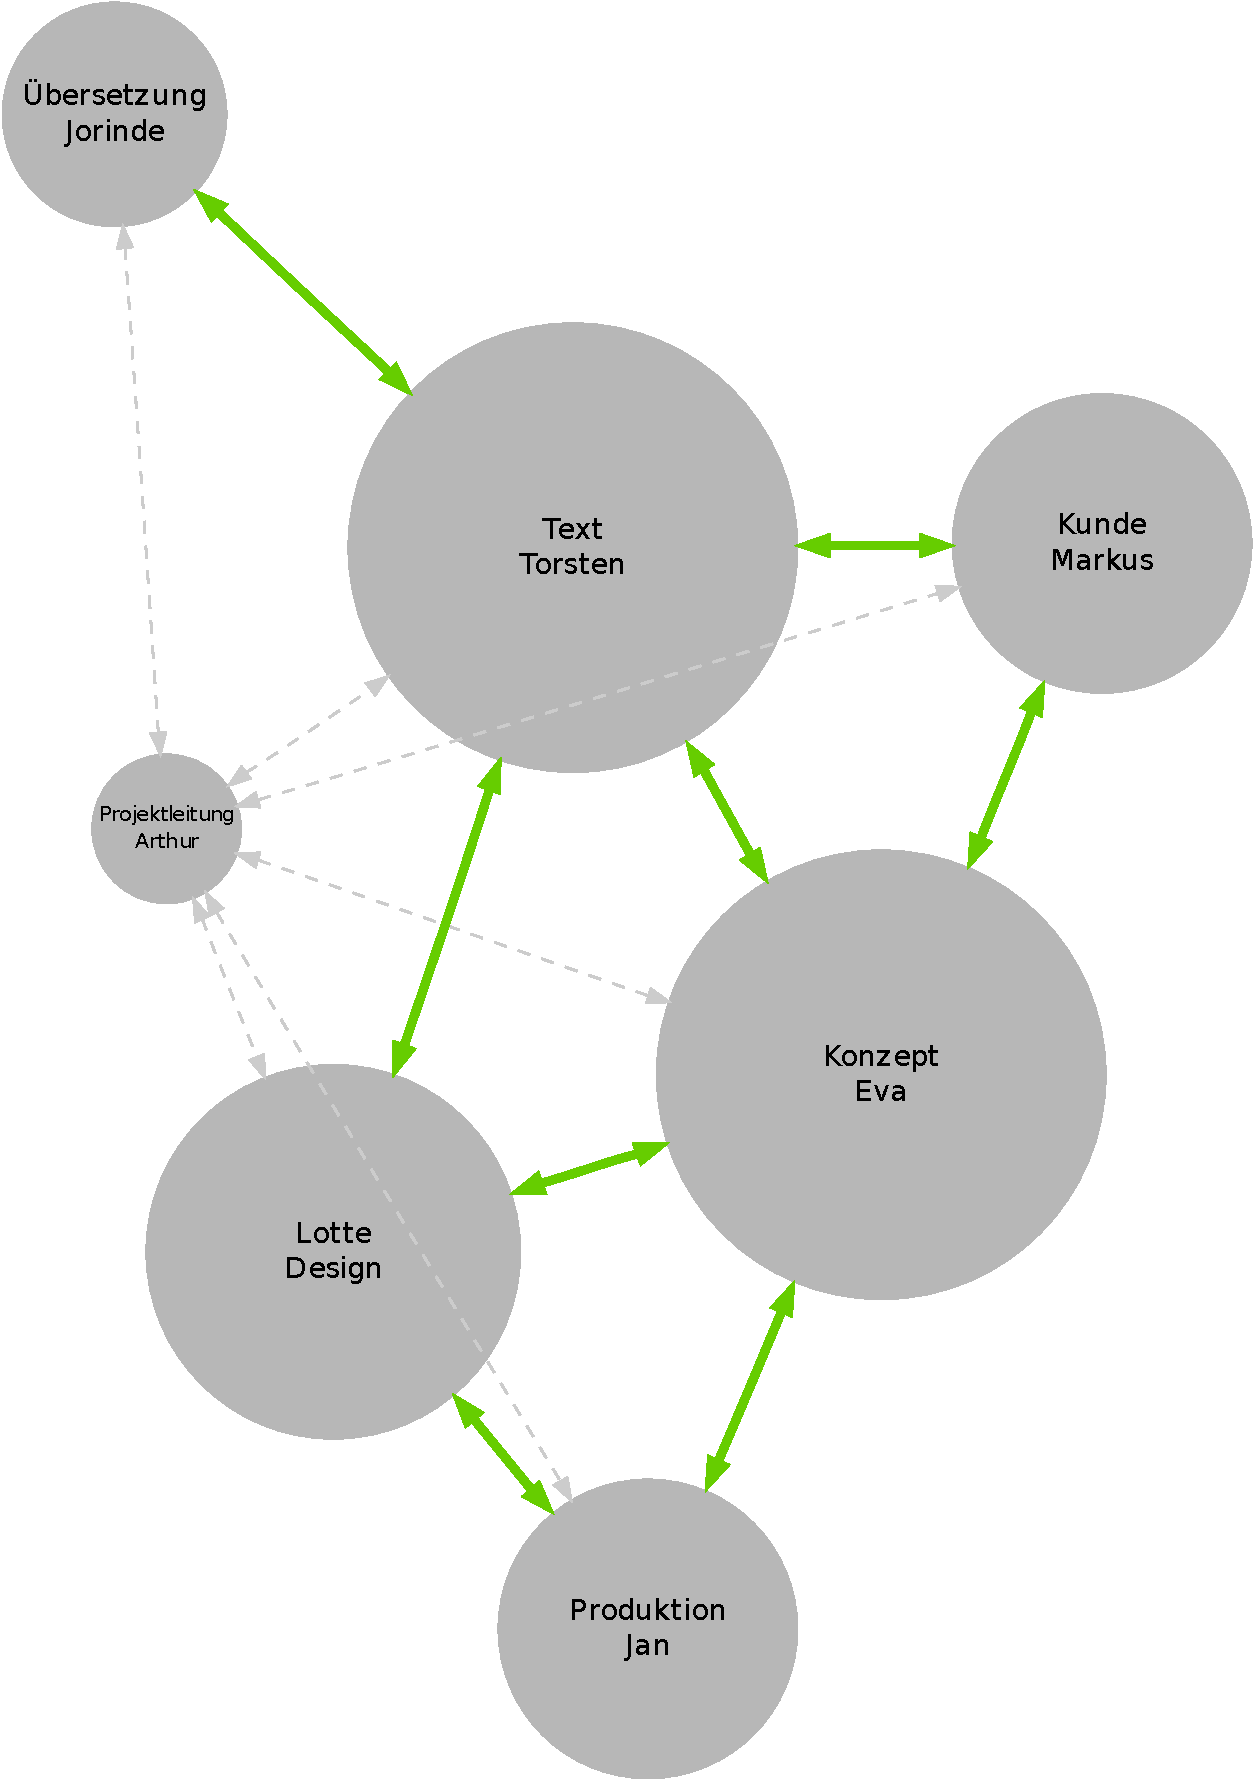
\includegraphics[width=0.85\textwidth]{media/personas-gewichtet.pdf}
\caption{Abstimmung zwischen den Personas bezogen auf Text, gewichtet nach Anzahl der Kommunikationspartner}
\label{chart:personas-gewichtet}
\end{center}
\end{figure}

\label{l:textattribute}

\paragraph{Typ} Überschrift, Untertitel, Bild-Beschreibung, Fließtext.

\paragraph{Workflow}

Beschreibung des optimalen Workflows und die Rolle der Beteiligten

Innerhalb der Anwendung wird das Projekt angelegt und die dafür benötigten Textbausteine definiert. Hierbei können detaillierte Angaben zu deren Eigenschaften gemacht werden, z.B. über den Verwendungszweck oder die maximal Länge. Die einzelnen Textbausteine werden bei diesem Vorgang entsprechend dem Aufbau des Endproduktes in eine Reihenfolge gebracht und hierarchisch angeordnet. So wird eine leichte Orientierung und Zuordnung der Text zum Endprodukt möglich. 

Nachdem die benötigten Textbausteine definiert wurden, werden diese durch Texter befüllt. Für Texter stellt die Anwendung Hilfsfunktionen zur Verfügung. Dazu zählen Informationen wie Zeichenlänge und Wortanzahl und Rechtschreibkorrektur mit Wörterbuch.

Sobald die Texte hinterlegt wurden durchlaufen sie die Qualitätskontrolle durch andere Mitarbeiter des Projektes und anschließend den Freigabeprozess beim Kunden. Wurden die Texte freigegeben, können die zusammengestellten Texte in das Endprodukt übernommen werden. 

Alle Vorgänge werden innerhalb der Anwendung protokolliert und sind so für jeden Beteiligten leicht nachvollziehbar. Aufgaben können automatisch aufgrund von Änderungen erzeugt werden, oder von Mitarbeiter angelegt werden. So wird sichergestellt, dass alle Projektmitarbeiter jederzeit über ihre Aufgaben bezüglich der Texte informiert sind, bei Änderungen die verantwortlichen Mitarbeiter informiert werden. Dadurch wird es möglich auch bei Korrekturen in letzter Minute diese Änderungen gezielt und transparent zu übernehmen.

